\paragraph{Create Event}
	\begin{figure}[H]
		\centering
		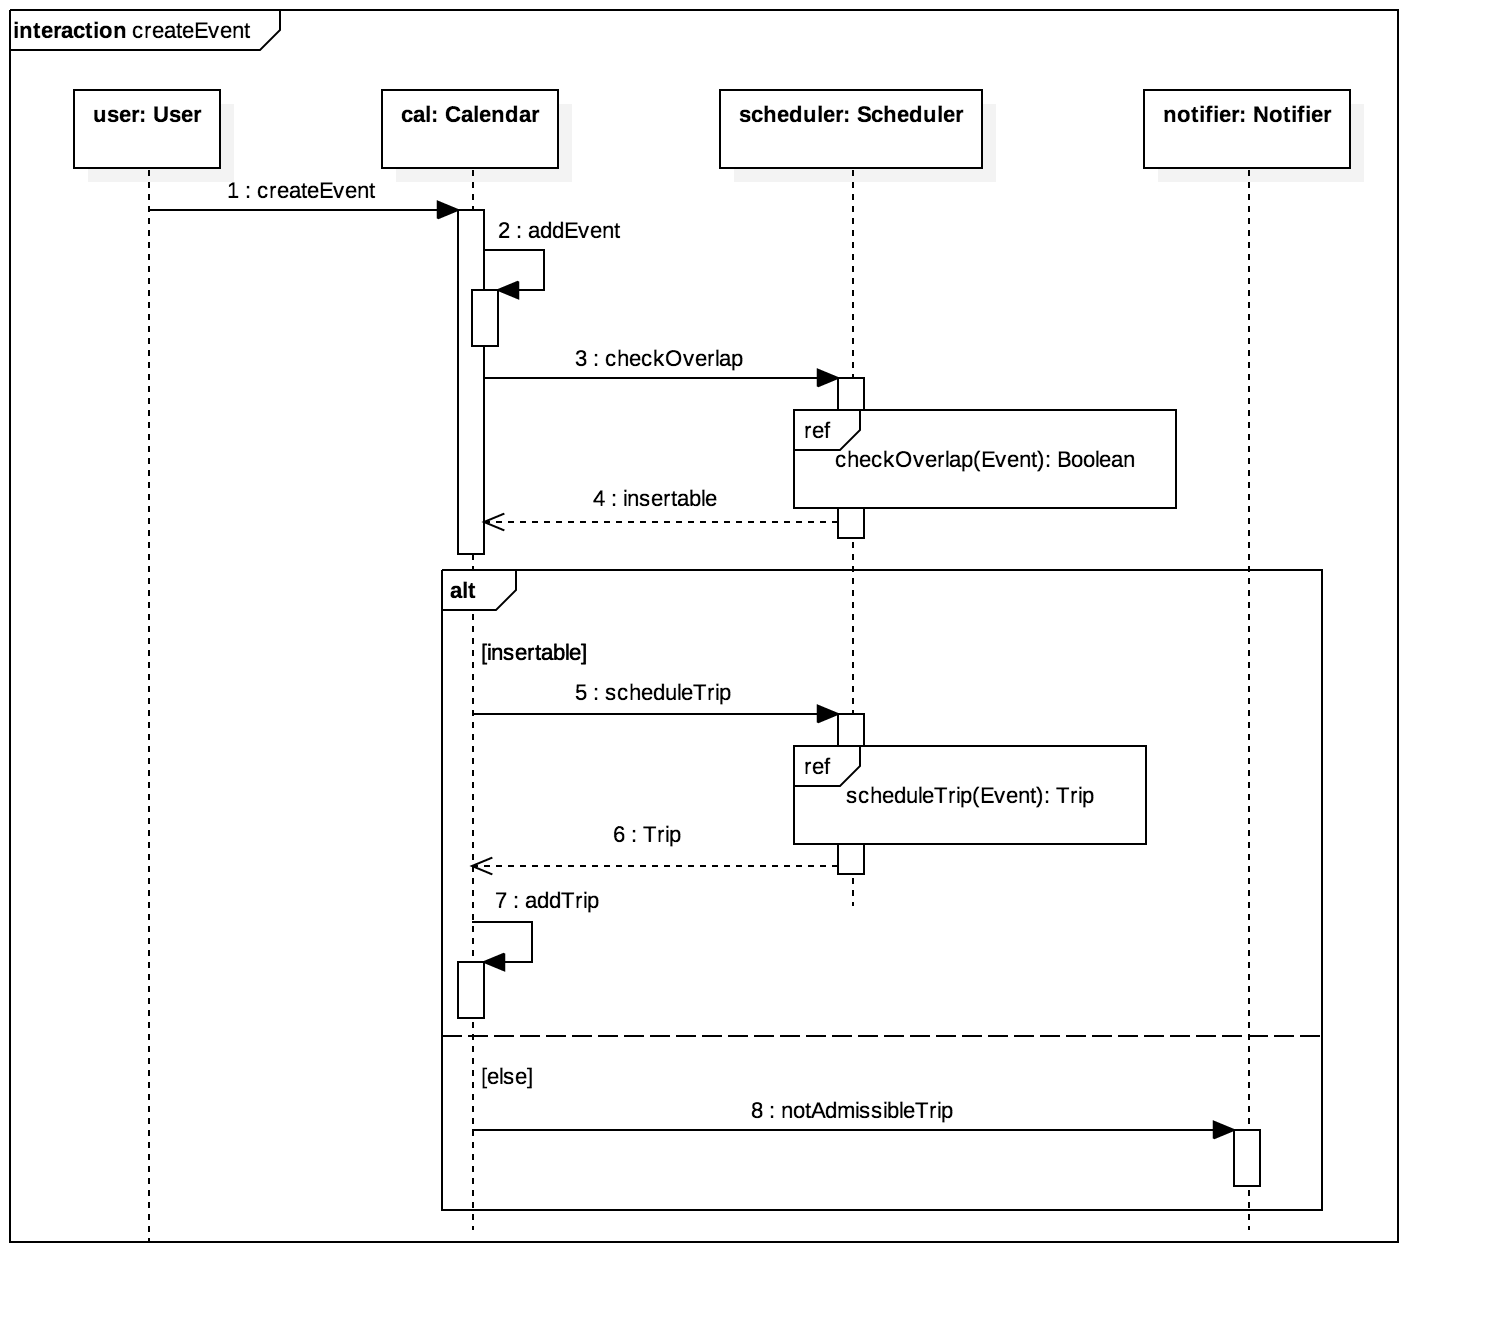
\includegraphics[width=\textwidth]{uml/sequenceDiagrams/createEvent}
		\caption{Create Event Sequence Diagram}
	\end{figure}
	\vfill
	
\paragraph{Subsquence: Check for Overlapping event}
	\begin{figure}[H]
		\centering
		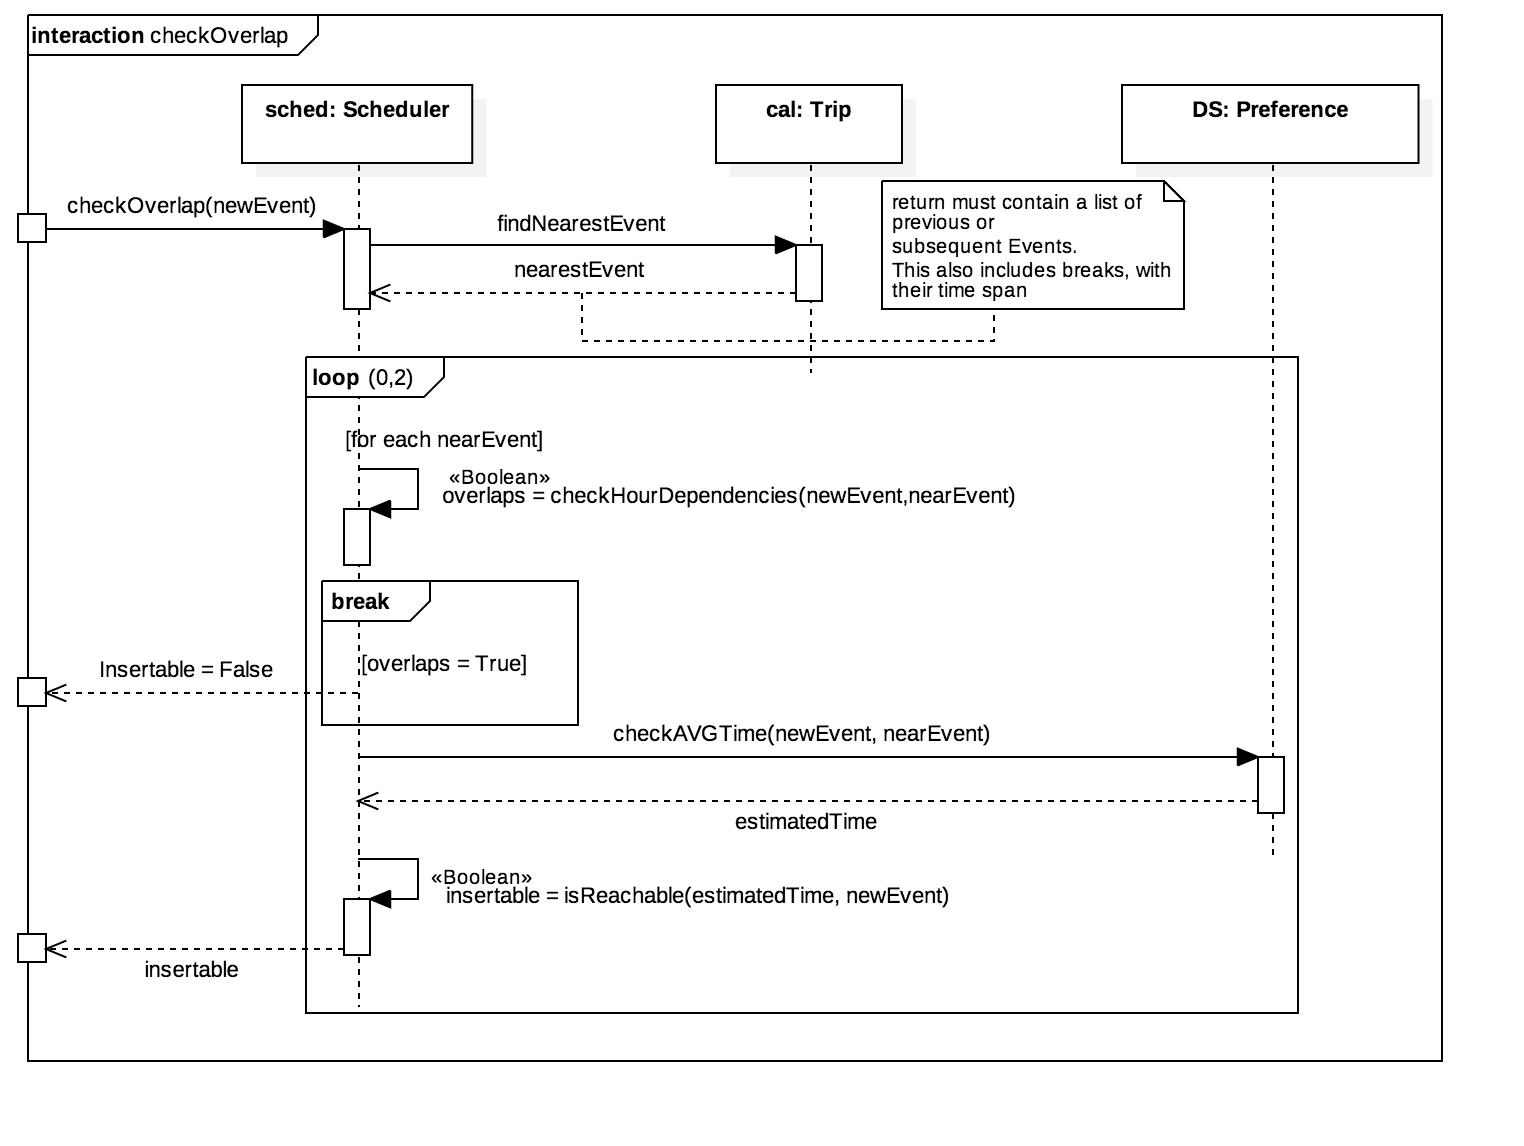
\includegraphics[width=\textwidth]{uml/sequenceDiagrams/checkOverlap}
		\caption{Check Overlap Sequence Diagram}
	\end{figure}
	\vfill
		
\paragraph{Subsquence: Schedule a Trip}	
	\begin{figure}[H]
		\centering
		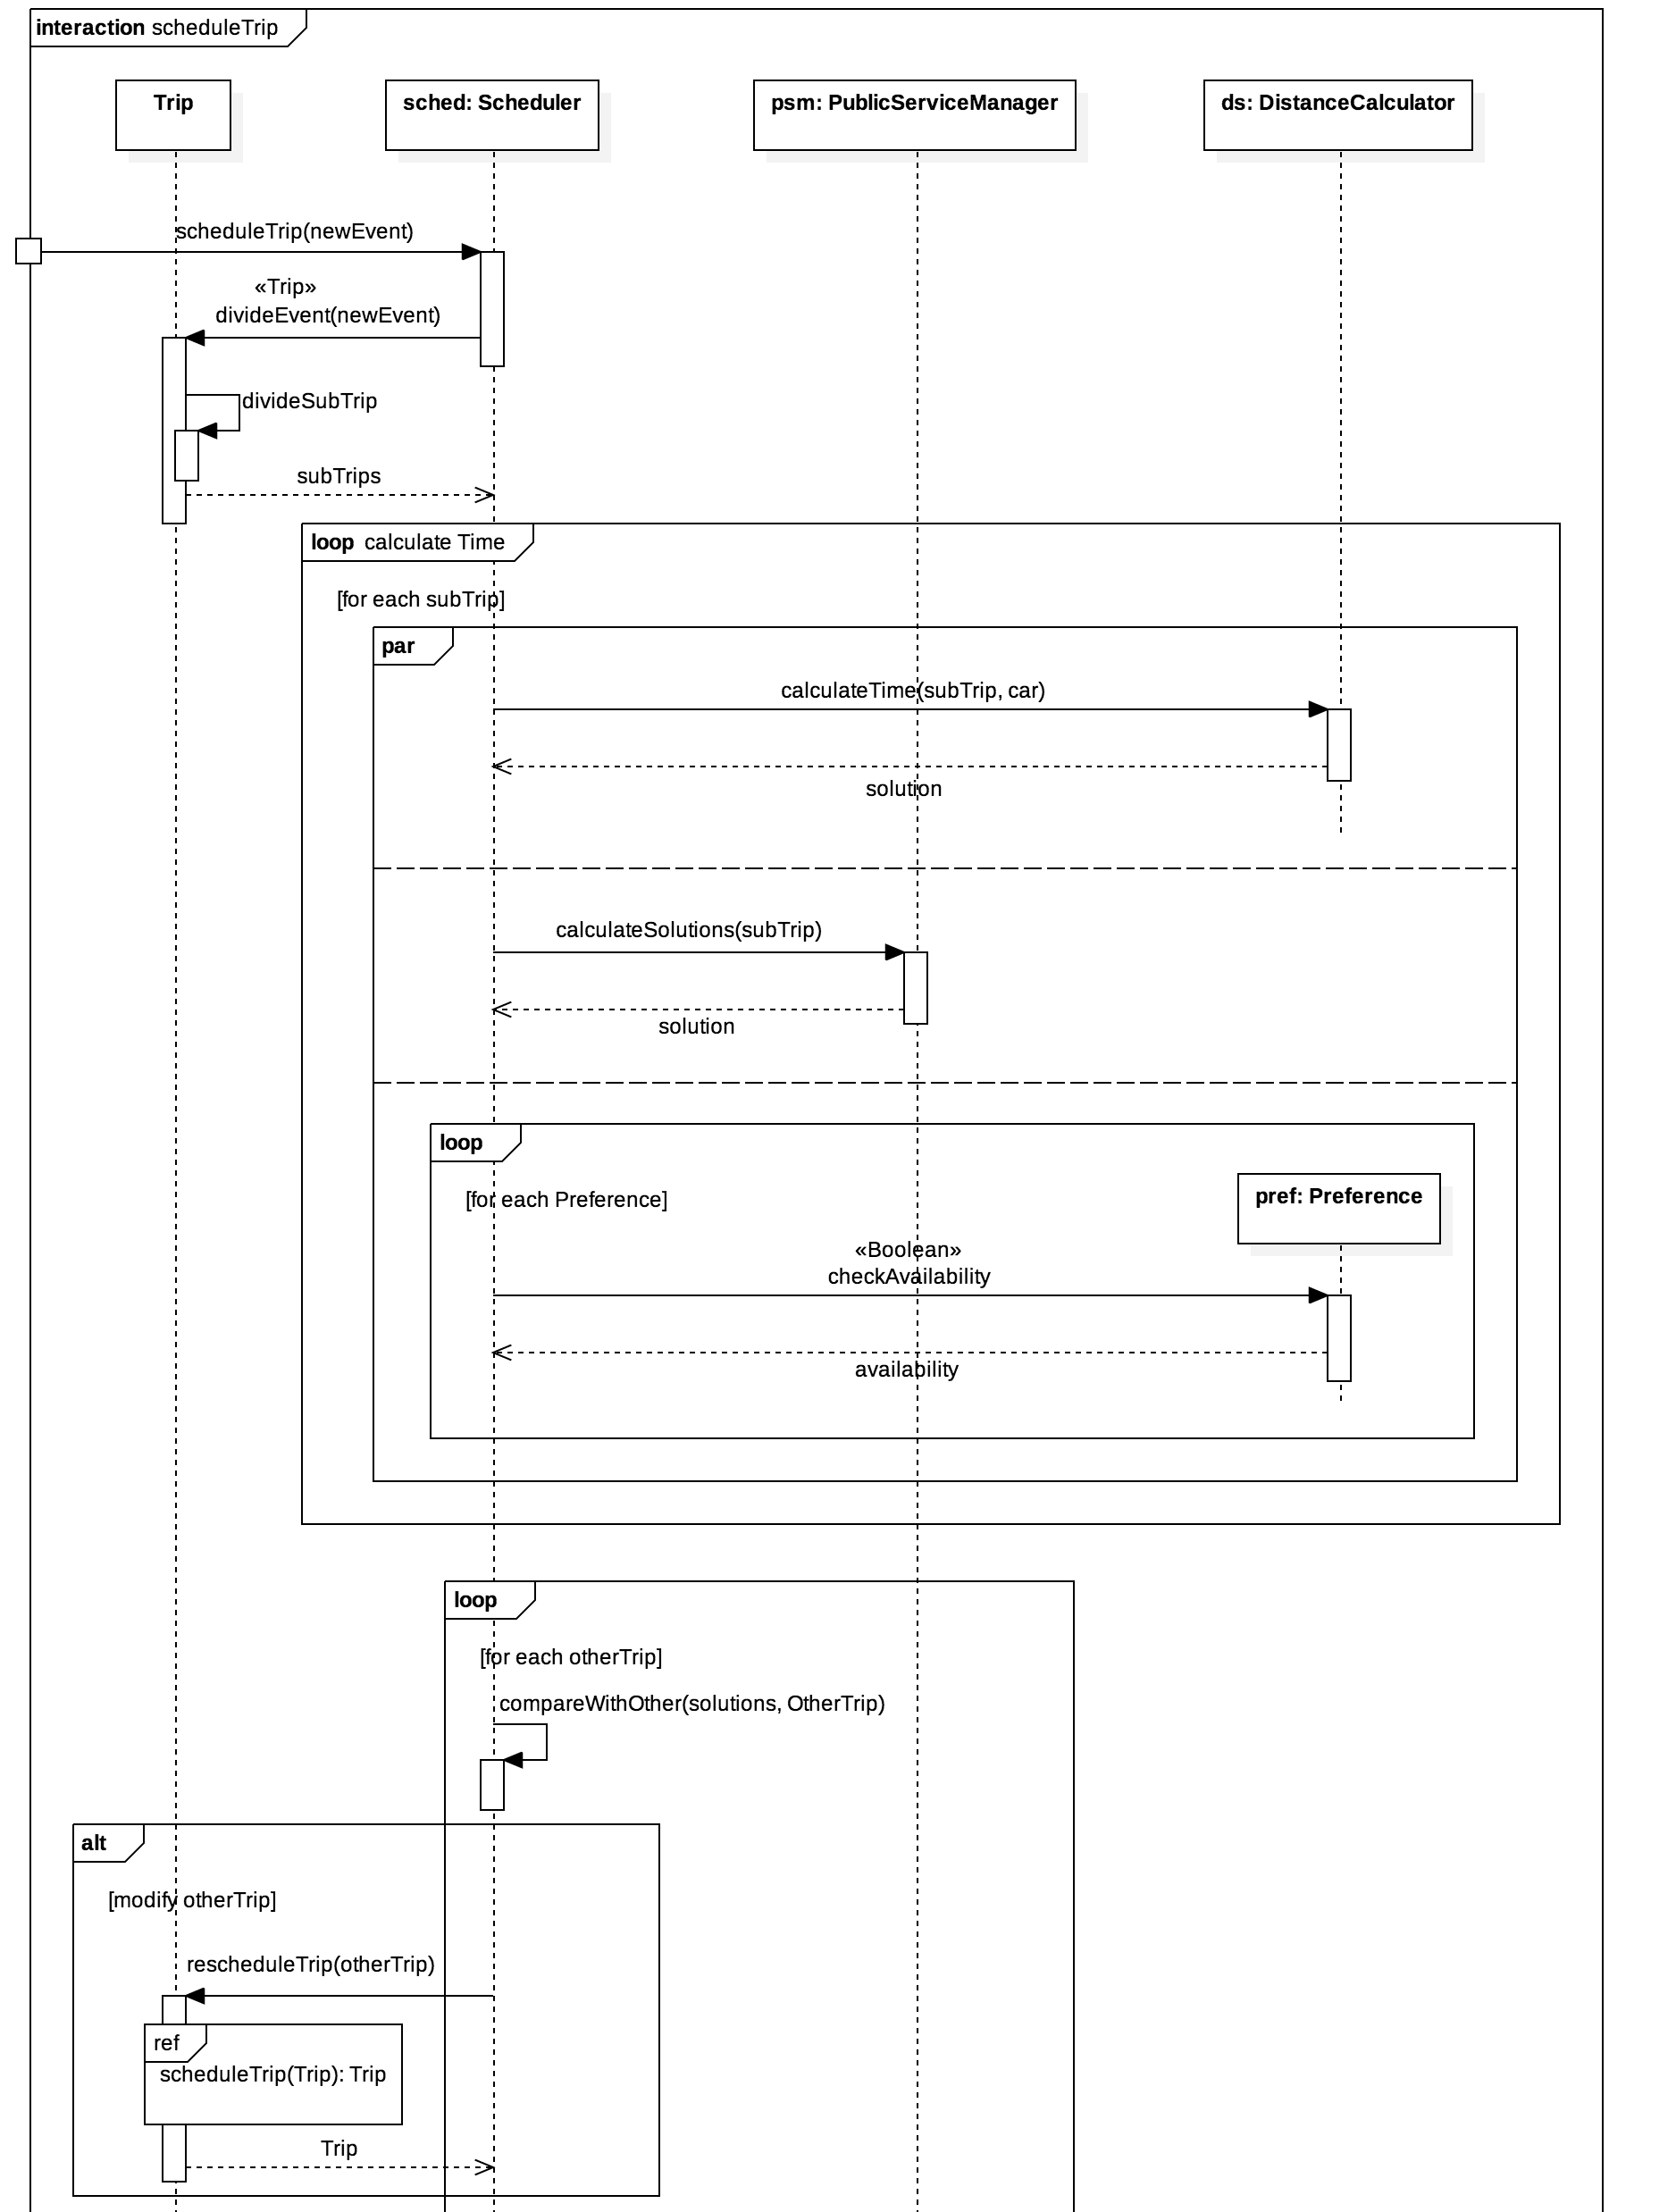
\includegraphics[width=\textwidth]{uml/sequenceDiagrams/scheduleTrip-part1}
		\caption{First Part of Trip Scheduling Sequence Diagram}
	\end{figure}
	
	\vfill
	
	\begin{figure}[ht!]\ContinuedFloat
		\centering
		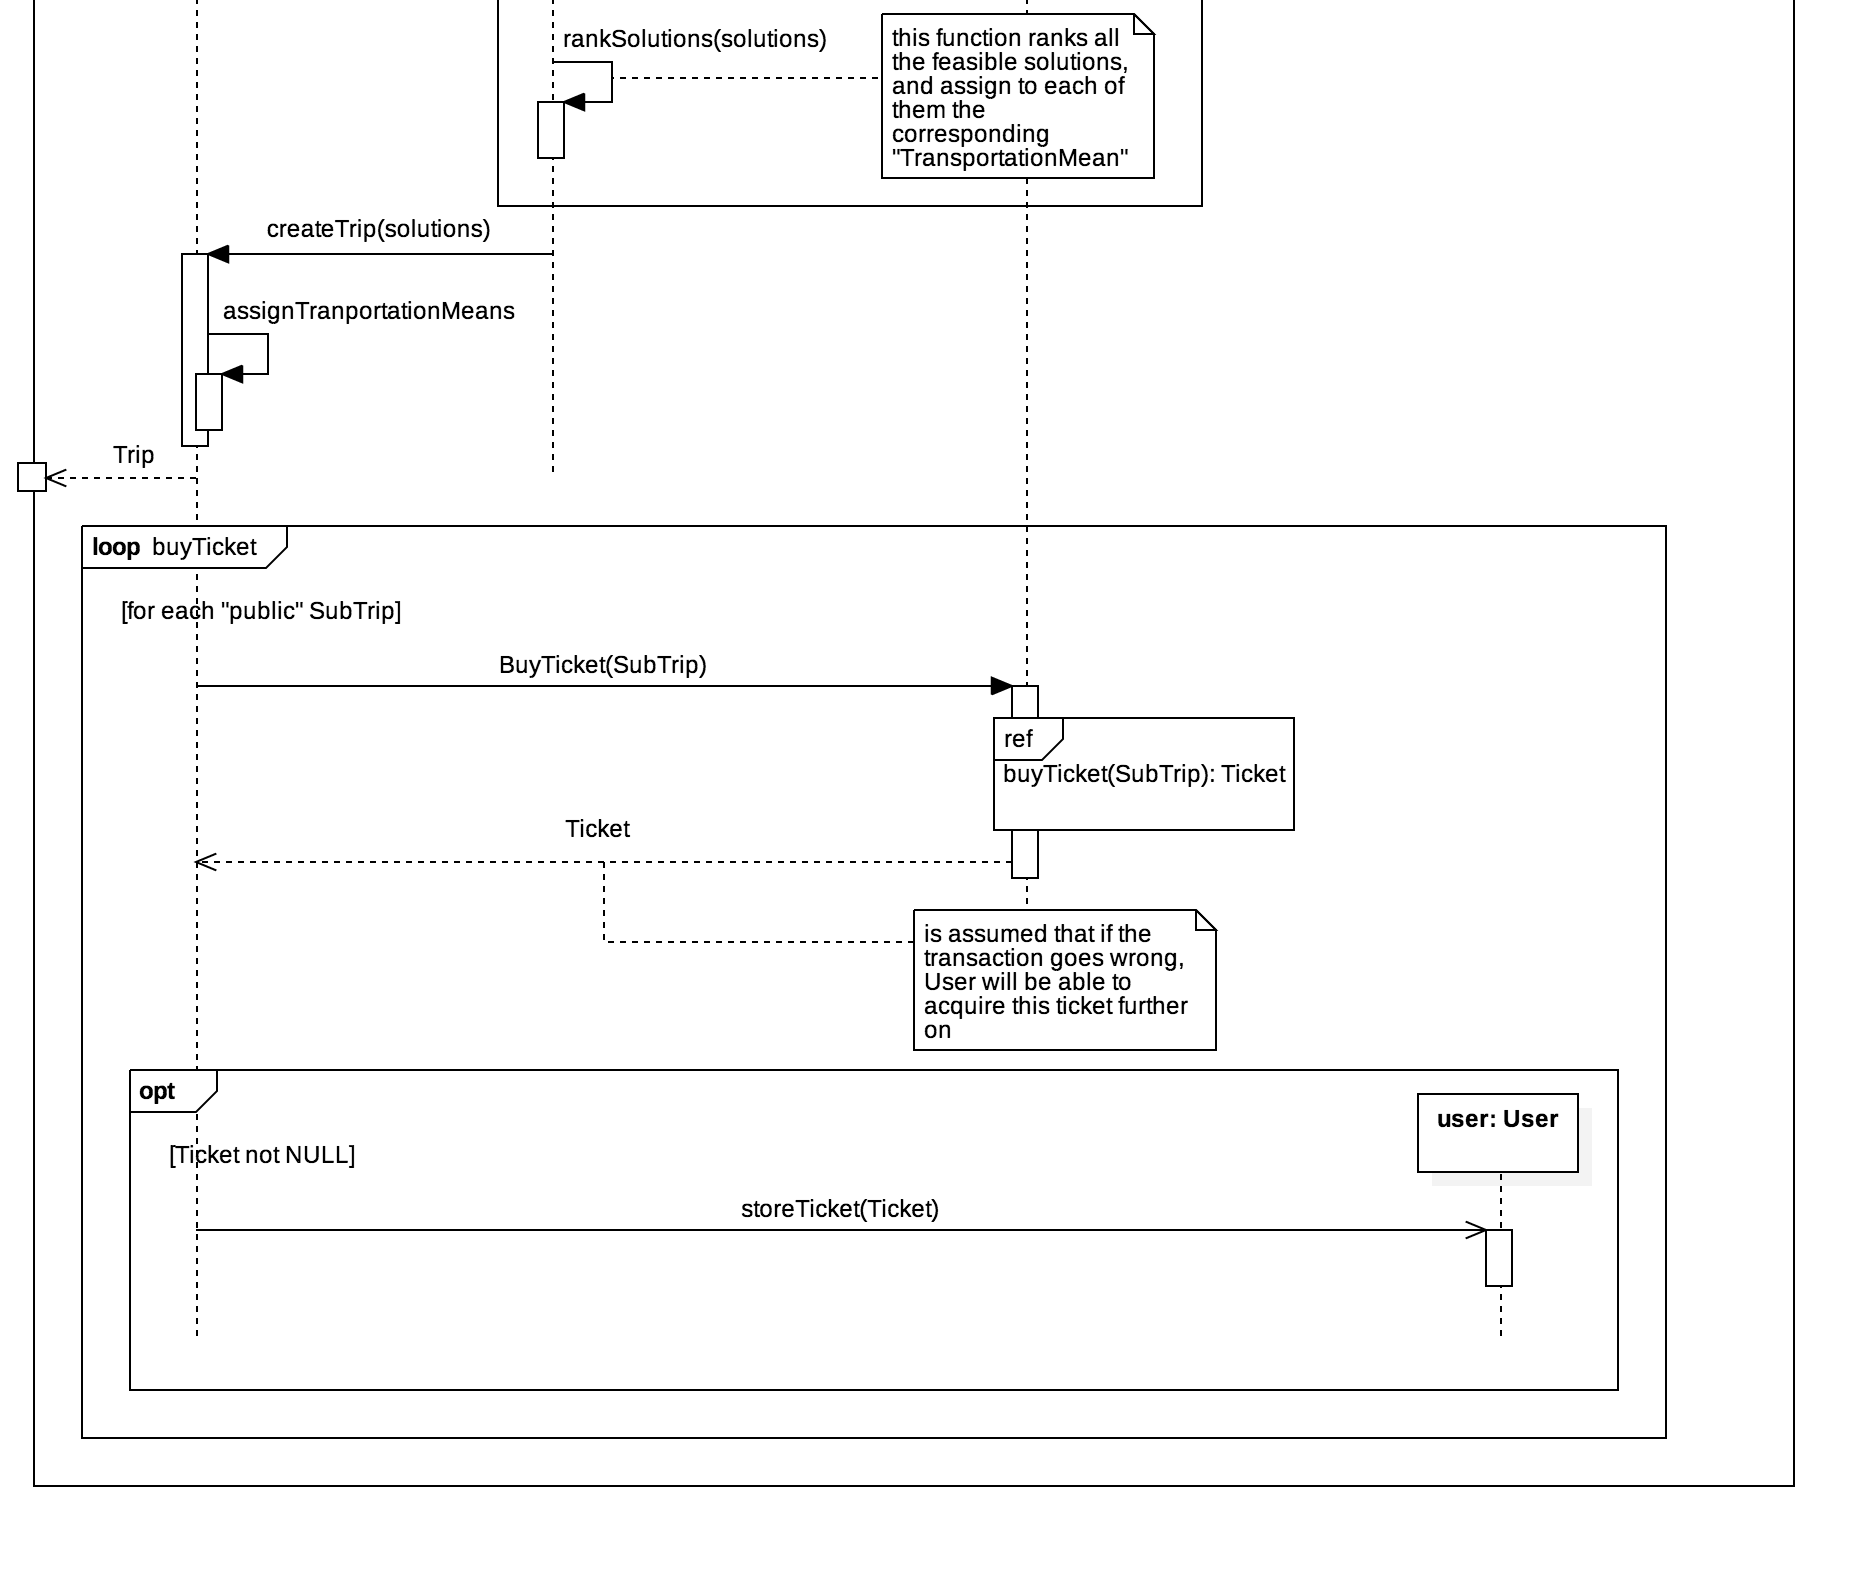
\includegraphics[width=\textwidth]{uml/sequenceDiagrams/scheduleTrip-part2}
		\caption{Second Part of Trip Scheduling Sequence Diagram}
		\label{loginRunTimeView}
	\end{figure}

	\vfill
	
\paragraph{Dynamic Navigation}	
	\begin{figure}[H]
		\centering
		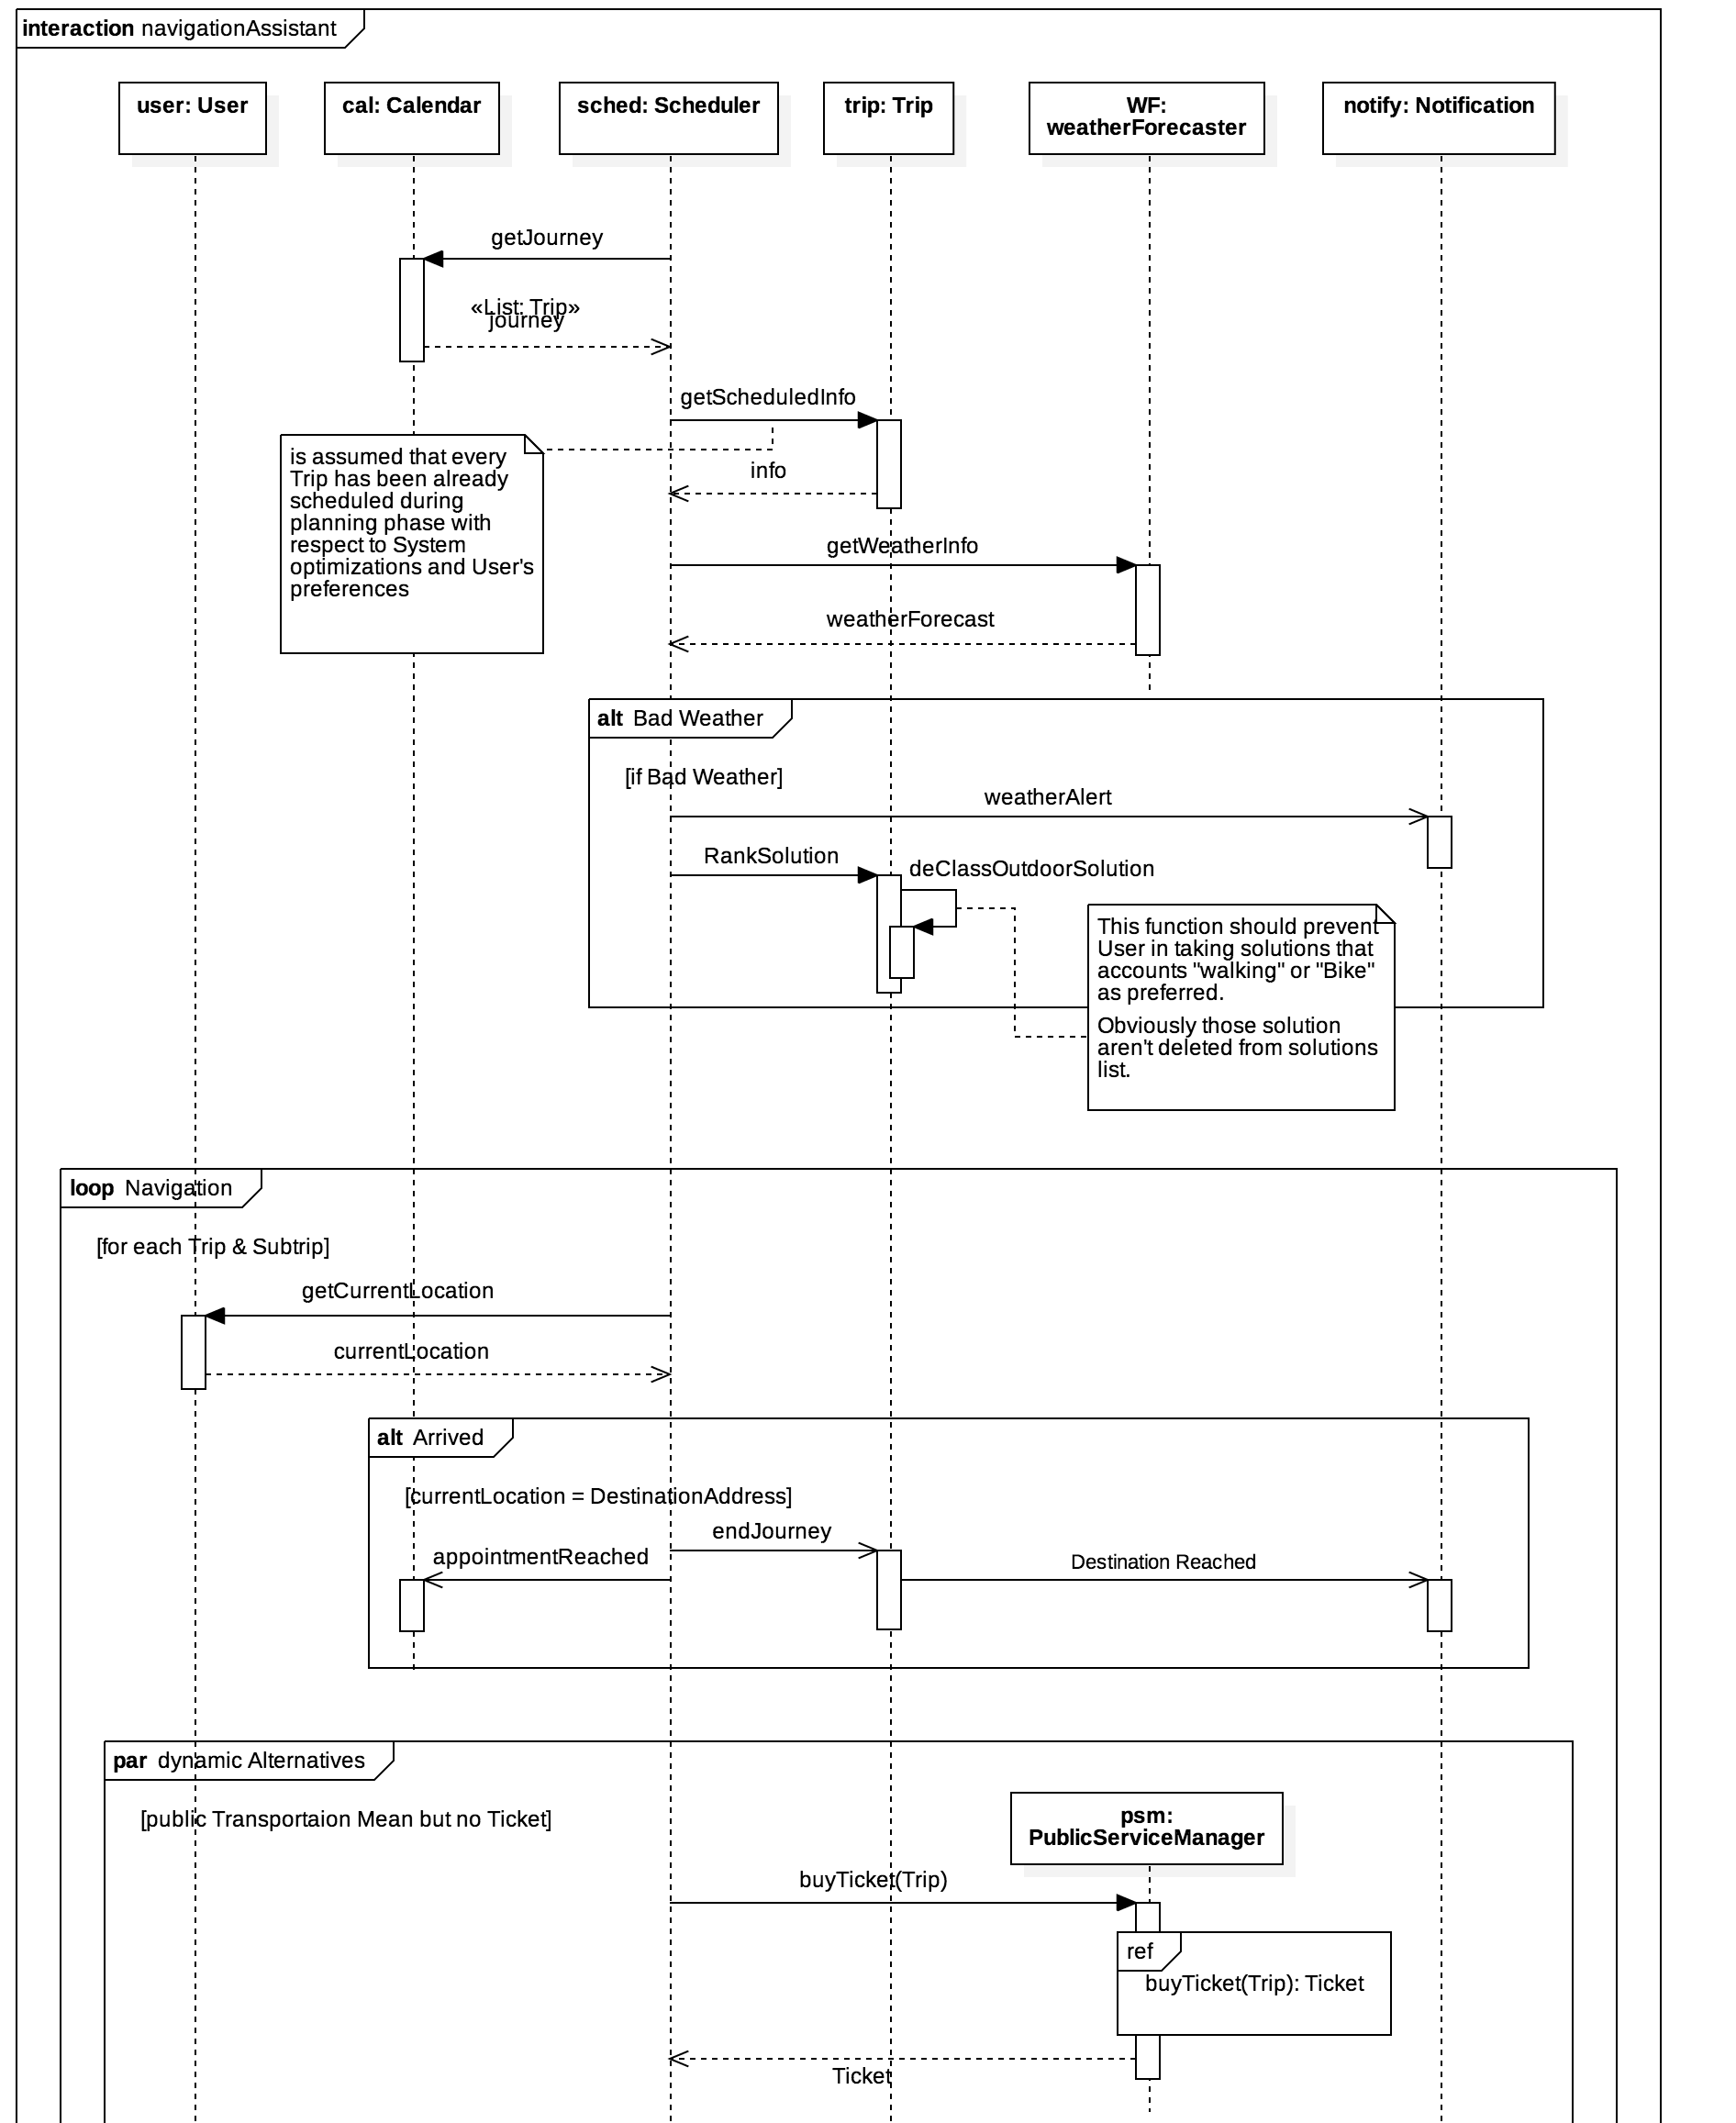
\includegraphics[width=\textwidth]{uml/sequenceDiagrams/navigationAssistant-part1}
		\caption{First Part of Dynamic Navigation Sequence Diagram}
	\end{figure}
	
	\vfill
	
	\begin{figure}[ht!]\ContinuedFloat
		\centering
		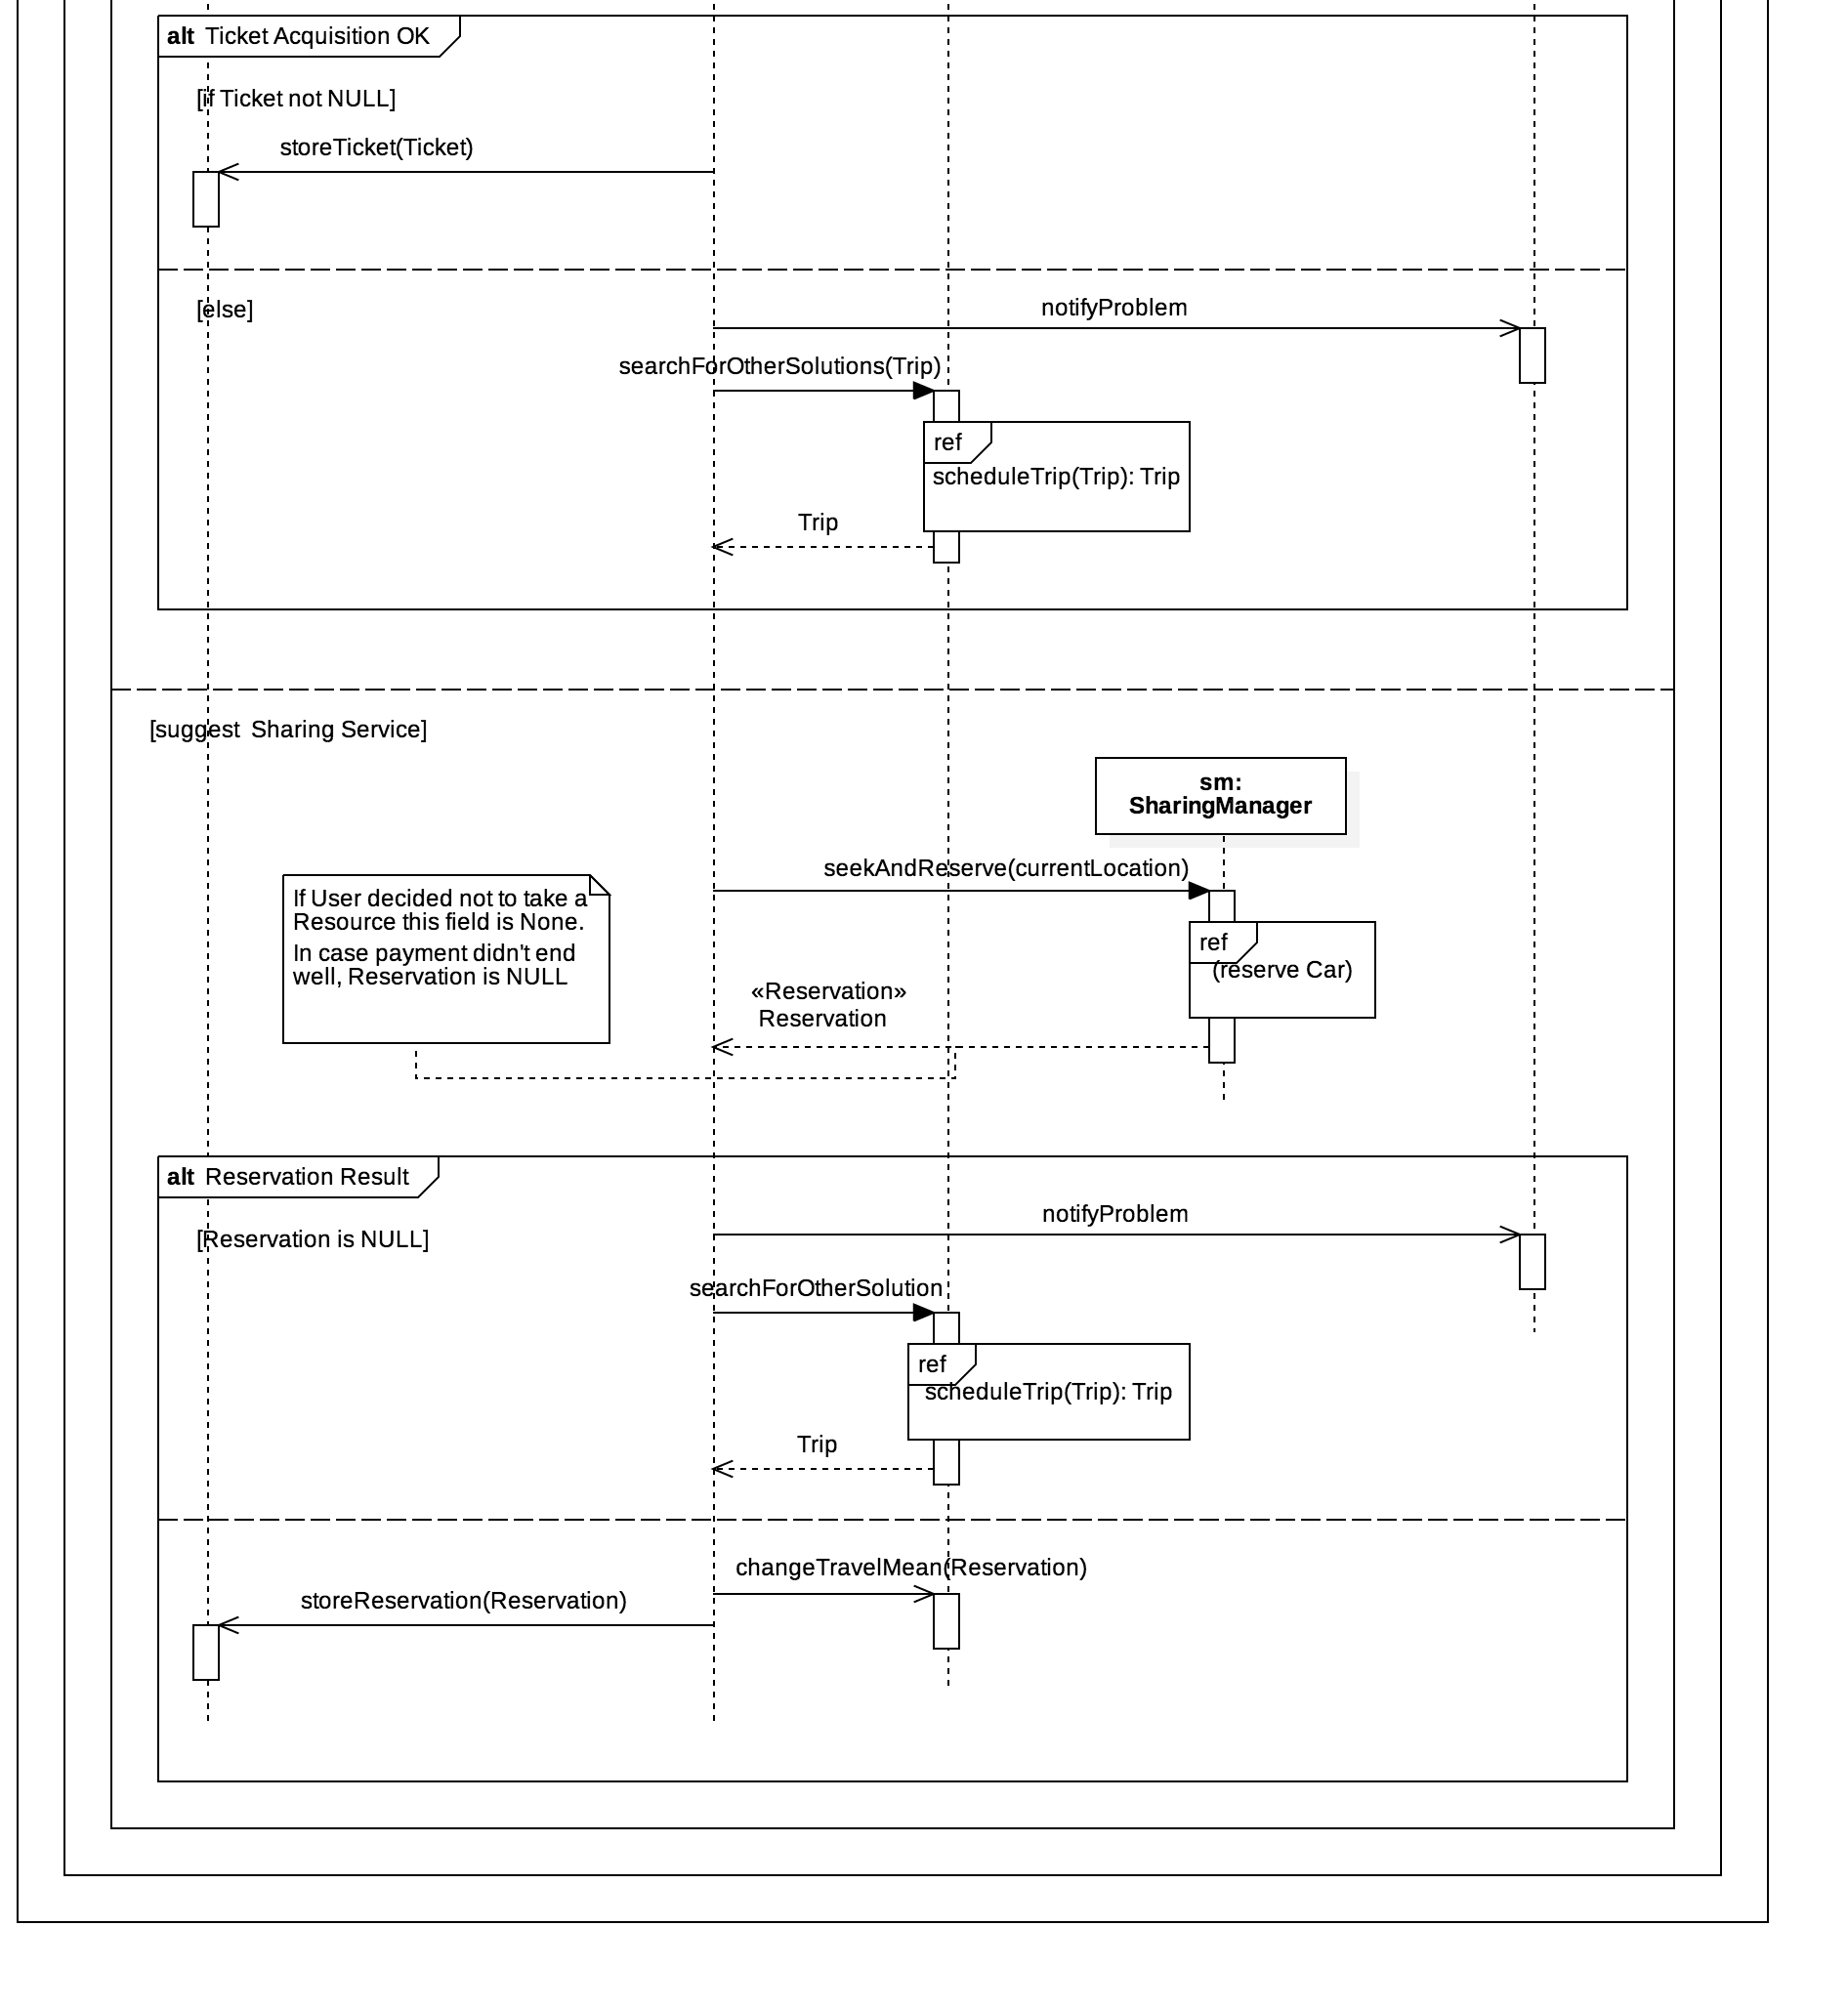
\includegraphics[width=\textwidth]{uml/sequenceDiagrams/navigationAssistant-part2}
		\caption{Second Part of Navigation Assistant Sequence Diagram}
		\label{loginRunTimeView}
	\end{figure}

	\vfill

\paragraph{Buy Public Tranportation Ticket}
	\begin{figure}[H]
		\centering
		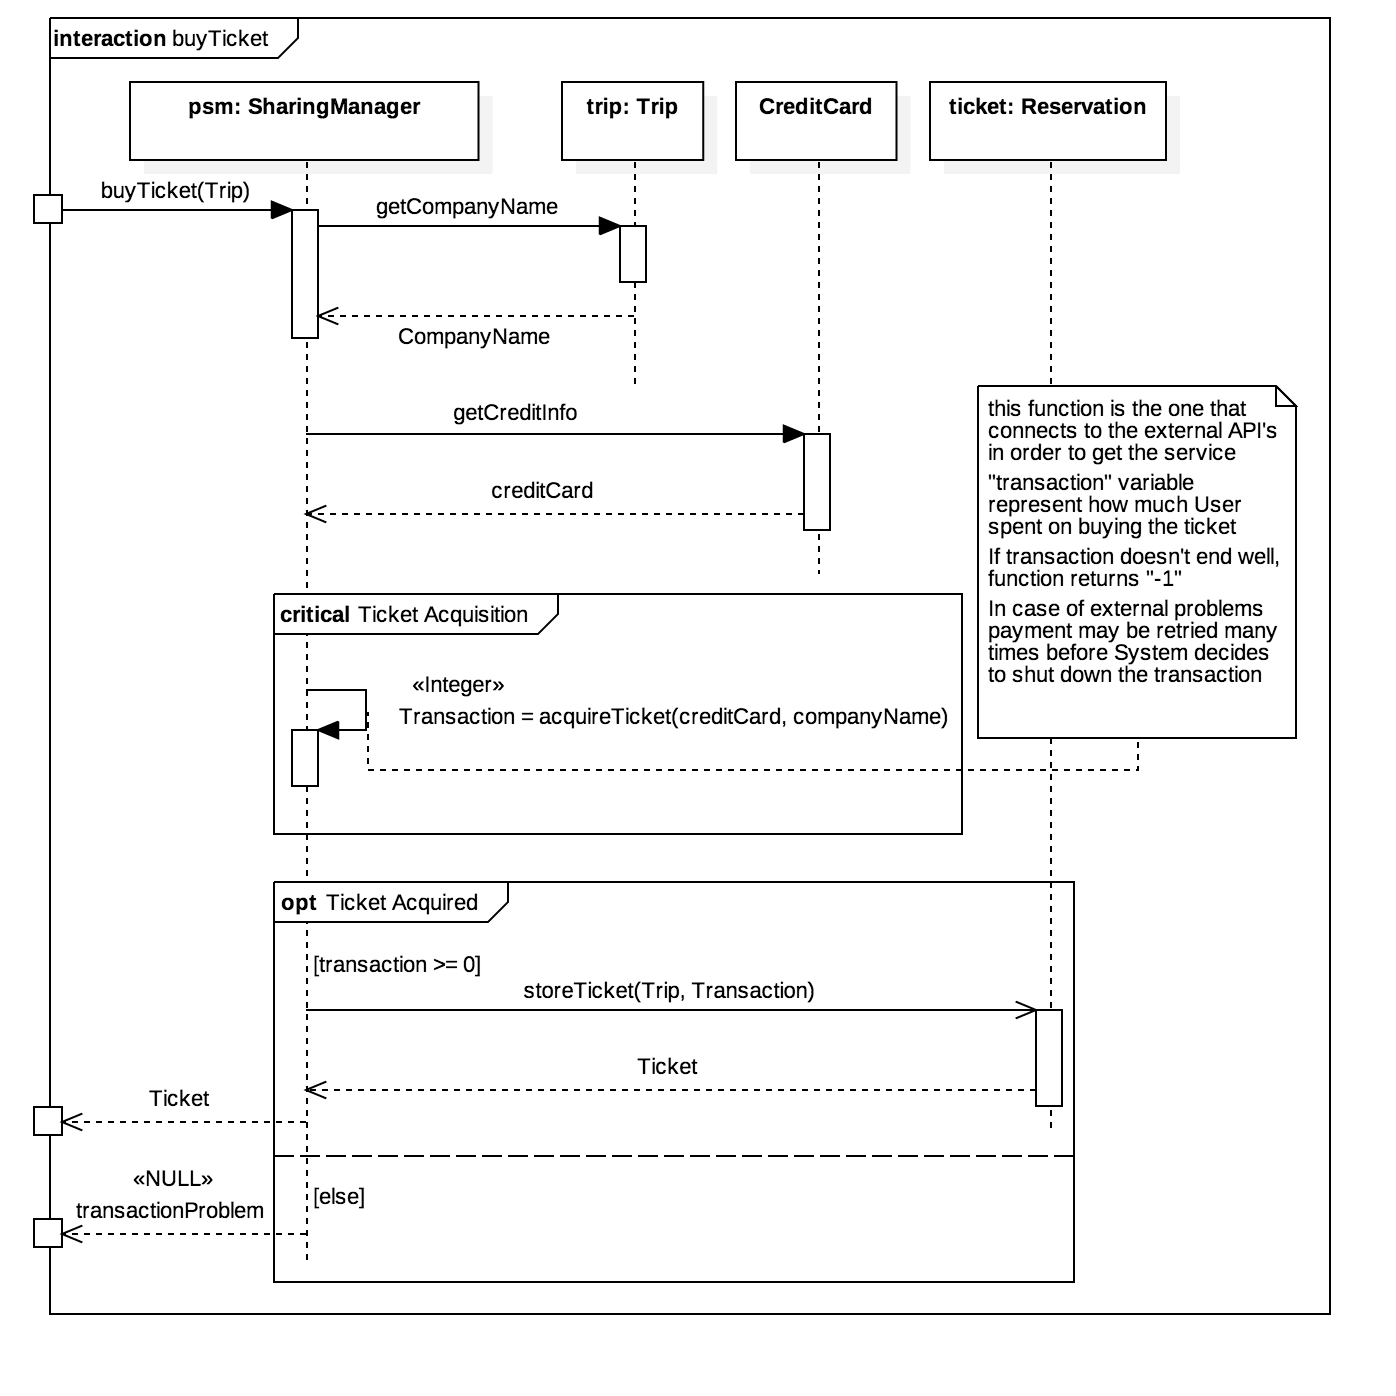
\includegraphics[width=\textwidth]{uml/sequenceDiagrams/buyTicket}
		\caption{Buy Public Tranportation Ticket Sequence Diagram}
	\end{figure}
	\vfill

\paragraph{Reserve Sharing Service Resource}
	\begin{figure}[H]
		\centering
		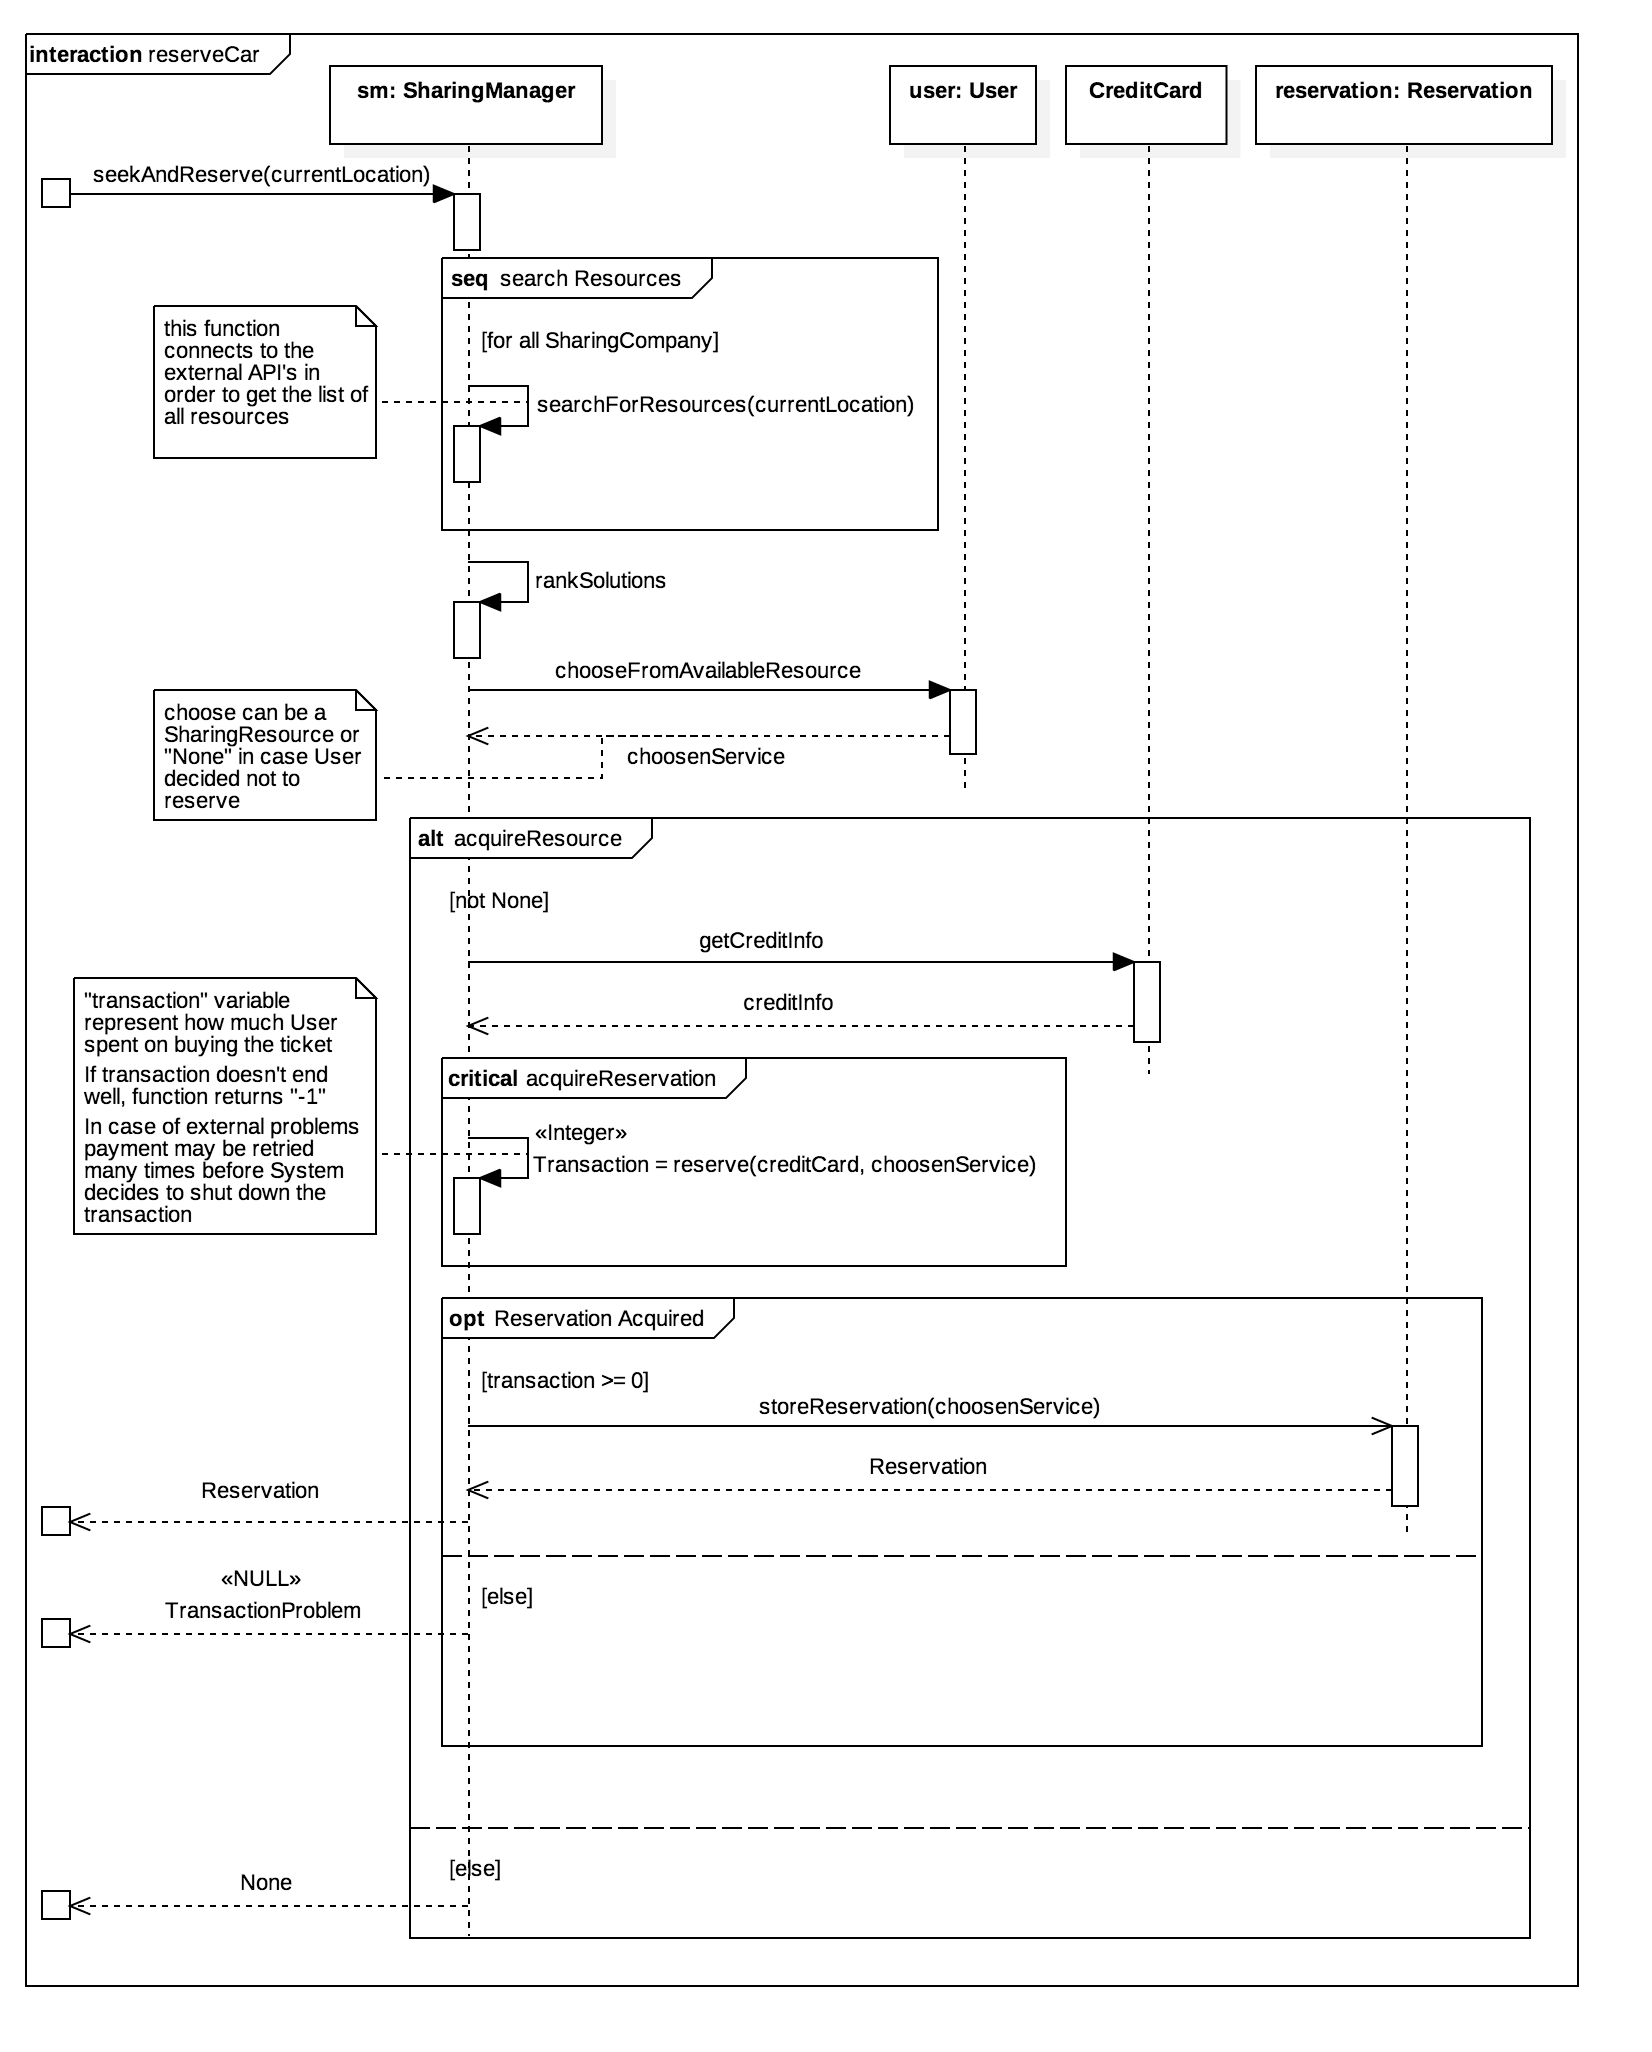
\includegraphics[width=\textwidth]{uml/sequenceDiagrams/reserveCar}
		\caption{Reserve Sharing Service Resource Sequence Diagram}
	\end{figure}
	\vfill
